% $Header: /Users/joseph/Documents/LaTeX/beamer/solutions/generic-talks/generic-ornate-15min-45min.de.tex,v 90e850259b8b 2007/01/28 20:48:30 tantau $

\documentclass{beamer}
\long\def\/*#1*/{}



\mode<presentation>
{
  \usetheme{Rochester}
}
\definecolor{MyBlue}{RGB}{0, 130 210}

\usepackage[german]{babel}
% oder was auch immer

\usepackage[latin1]{inputenc}
% oder was auch immer

\usepackage{times}
\usepackage[T1]{fontenc}
% Oder was auch immer. Zu beachten ist, das Font und Encoding passen
% m�ssen. Falls T1 nicht funktioniert, kann man versuchen, die Zeile
% mit fontenc zu l�schen.


\title[University of Amsterdam] % (optional, nur bei langen Titeln n�tig)
{TERESA : Telepresence Reinforcement Learning Social Agent.}

\subtitle
{WP5 : Learning Social Skills} % (optional)

\author[Kyriacos Shiarlis] % (optional, nur bei vielen Autoren)
{Kyriacos Shiarlis}
% - Der \inst{?} Befehl sollte nur verwendet werden, wenn die Autoren
%   unterschiedlichen Instituten angeh�ren.

\institute[University of Amsterdam] % (optional, aber oft n�tig)
{University of Amsterdam}
% - Der \inst{?} Befehl sollte nur verwendet werden, wenn die Autoren
%   unterschiedlichen Instituten angeh�ren.
% - Keep it simple, niemand interessiert sich f�r die genau Adresse.

\date[] % (optional)
{16/06/2014}

\AtBeginSection[]
{
  \begin{frame}<beamer>{}
    \tableofcontents[currentsection]
  \end{frame}
}


% Falls Aufz�hlungen immer schrittweise gezeigt werden sollen, kann
% folgendes Kommando benutzt werden:

%\beamerdefaultoverlayspecification{<+->}



\begin{document}



\begin{frame}
  \titlepage
\end{frame}

\begin{frame}{}
  \tableofcontents[]
  % Die Option [pausesections] k�nnte n�tzlich sein.
\end{frame}

%% GENERAL PROJECT DESCRIPTION - - - - - - - - - - - - - - - - - - - - - - - - - - - - - - - - - - - - - - - - - - - - - - 
\section{The Project}
\begin{frame}{Telepresence - What?}
	\begin{center}
	 Remotely controlled robots that allow the user to interact with an environment, without being physically present.
	 
	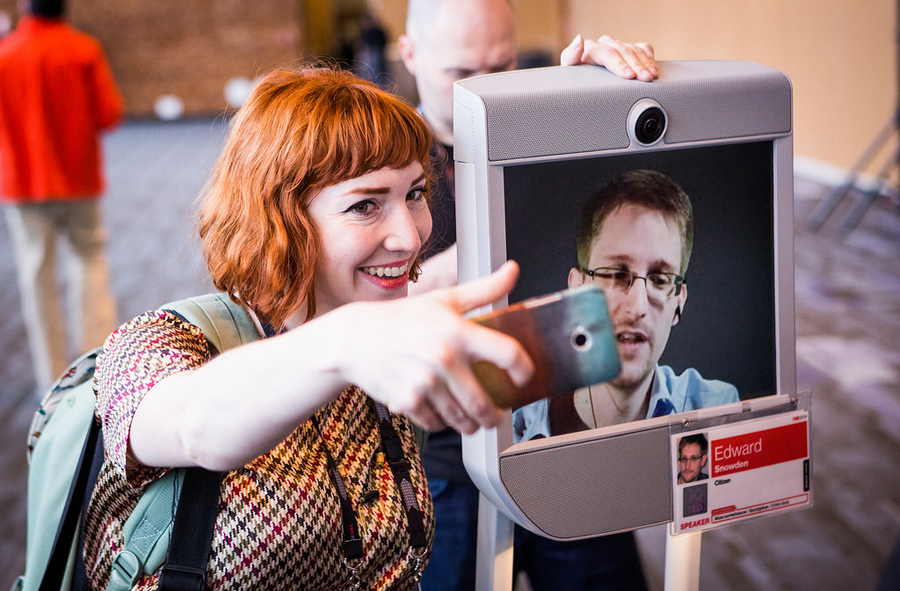
\includegraphics[scale = 0.4]{SNOW.jpg}		
	\end{center}
\end{frame}
% PROJECT MOTIVATION
\begin{frame}{Telepresence - Why?}
Telepresence allows greater remote user \textbf{control} and \textbf{interaction}.

User also \textbf{feels} and \textbf{appears} more present in a remote situation.\\
\vspace{3mm}
\underline{Applications include:}
	\begin{itemize}
		\item \textbf{Assistive technologies:} Remote visits to elderly, disabled, or hospitalised individuals.	
		\item \textbf{Industrial:} Remote inspections, conferences, visits.
		\item \textbf{Academic:} Conferences, supervisions. 
	\end{itemize}
			\setbeamercolor{postit}{fg=white,bg=MyBlue}
			\begin{beamercolorbox}[sep=0.5em,wd=10cm]{postit}
			TERESA concentrates on deployment in elderly homes.
		\end{beamercolorbox}
\end{frame}

% WHATS MISSING
\begin{frame}{Limitations}
	\begin{columns}
		\begin{column}[t]{5cm}
			\begin{figure}
				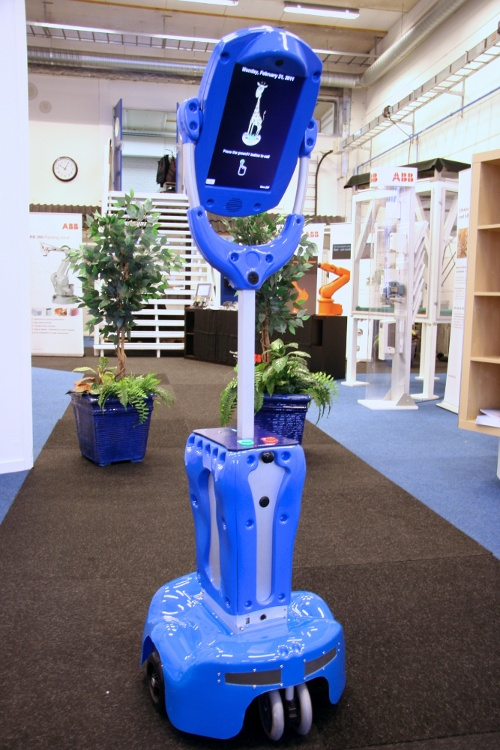
\includegraphics[width = 35mm, height =50mm]{ROBOT.jpg}
			\end{figure}
		\end{column}
		\begin{column}[t]{6cm}
			\begin{itemize}
				\item \textbf{Control} of the device can be hard.\\
				\item Interaction is not as \textbf{natural} as a result.\\
				\item Device only allows \textbf{audiovisual} interaction.\\
			\end{itemize}
		\end{column}
	\end{columns}
\end{frame}

% PROJECT AIMS
\begin{frame}{Project Aims}
	\begin{block}{Practical}
		\begin{itemize}
			\item Remove the cognitive load of control.
			\item Appearing as human as possible. 
		\end{itemize}
	\end{block}
	\begin{block}{Scientific}
		\begin{itemize}
			\item To what extent socially acceptable behaviour can be Learned.
			\item What sort of implicit feedback is needed to achieve this.
		\end{itemize}
	\end{block}
\end{frame}


% EXAMPLE
\begin{frame}{Example}
	\begin{block}{Questions}
		How should a robot approach a group of people? What what is the correct distance to stop?
	\end{block}
	$\Rightarrow$ Hard Coding Social Norms is very complex.
	\begin{block}{Our approach}
		Experiment $\rightarrow$ Data $\rightarrow$ Offline Learning $\rightarrow$ Implicit Reward  $\rightarrow$ Semi-autonomous behaviour.	
	\end{block}
	$\Rightarrow$ Easier and more natural local-remote user interaction.
\end{frame} 

% CONGITIVE ARCHITECTURE
\begin{frame}{Cognitive Architecture}
	\begin{center}
		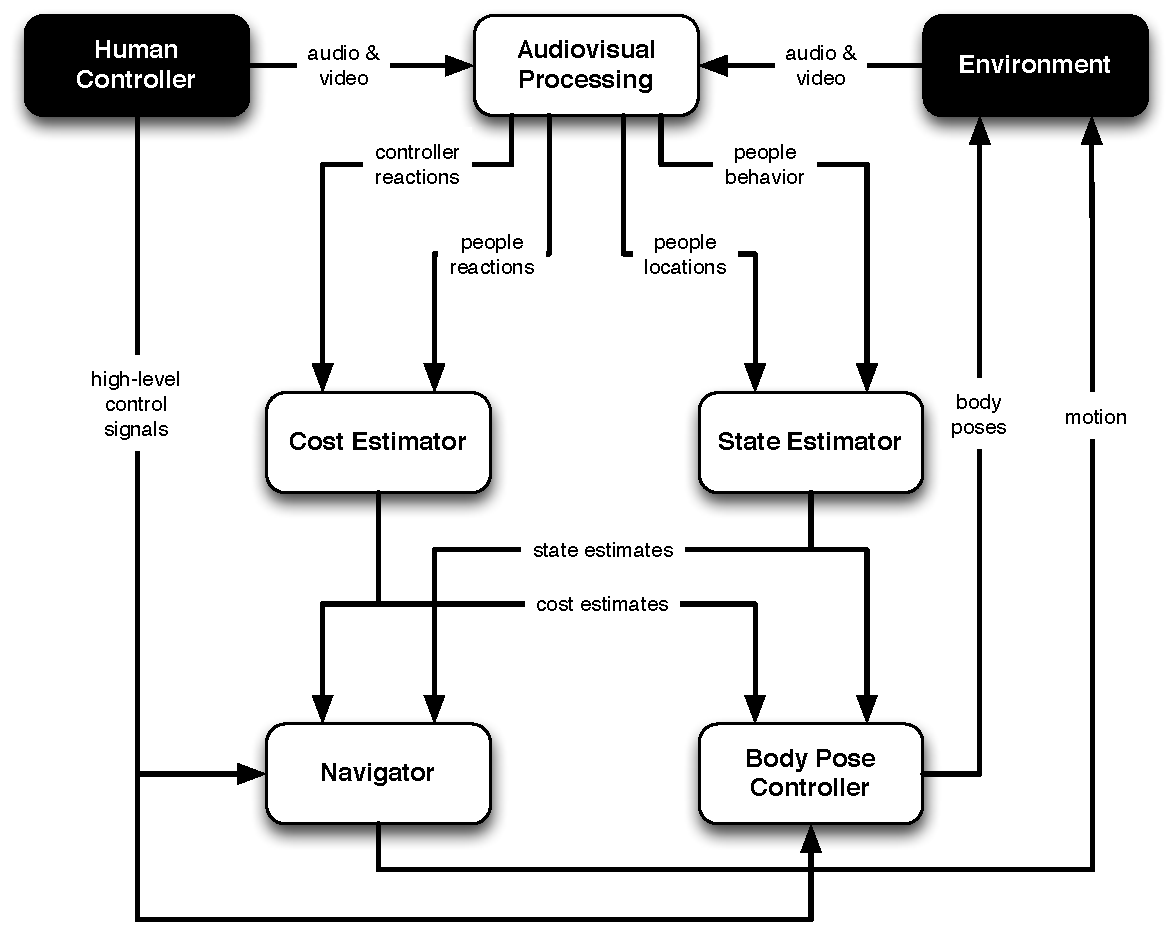
\includegraphics[scale = 0.45]{framework.pdf}
	\end{center}
\end{frame}

%% Learning Social Skills - - - - - - - - - - - - - - - - - - - - - - - - - - - - - - - - - - - - - - - - - - - - - - - - - - - - - - - - -
%Questions
\section{Learning Social Skills}
\begin{frame}{Learning Social Skills}
	How can emotional feedback from the robot's environment improve its behaviour?\\
	\begin{block}{Example}
		Robot comes \textbf{dangerously} close and at high velocity - Person \textbf{frowns} - After learning the robot \textbf{avoids} action in similar situations. 	
	\end{block}
	Does that perform better than hand-coding social behaviour?		
\end{frame}

% AIMS
\begin{frame}{Learning Social Skills - Aims}
	\begin{center}
		\begin{columns}
			\begin{column}[t]{3cm}
				\underline{\textbf{Extract}}
			\end{column}
			\begin{column}[t]{2cm}
				\underline{\textbf{Integrate}}
			\end{column}
			\begin{column}[t]{1cm}
				\underline{\textbf{Plan}}
			\end{column}
		\end{columns}
	\end{center}
	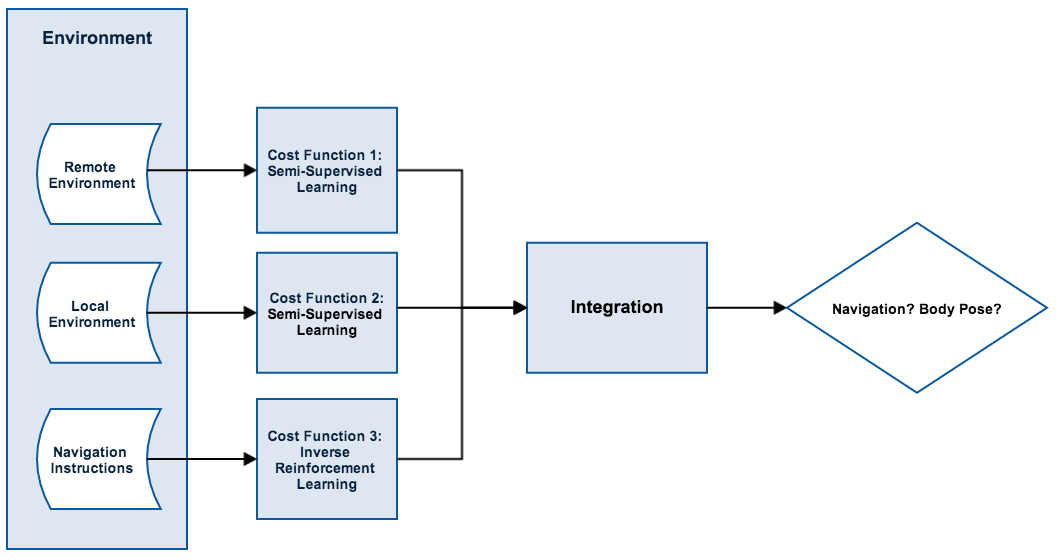
\includegraphics[scale = 0.29]{MODULES.png}
\end{frame}

%Extract
\begin{frame}{Challenges}
	\begin{block}{Extraction}	
		Extracting reward from the environment is an exercise in implicit feedback.
		\begin{itemize}
			\item Semi-Supervised Learning : Implicit emotional state $\Rightarrow$ Reward.			
			\item Inverse Reinforcement Learning: Expert trajectories $\Rightarrow$ Reward
		\end{itemize}
	\end{block}
	\begin{center}
		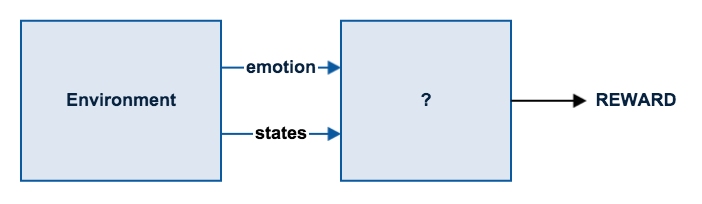
\includegraphics[scale = 0.4]{EXTRACT.png}
	\end{center}
\end{frame}
\begin{frame}{Challenges}
	\begin{block}{Integration}
		Integration of cost functions should be done intelligently.
		\begin{itemize}
			\item Could be based on individual function confidence.
			\item Bayesian Approach.
		\end{itemize}
	\end{block}
	\begin{center}
		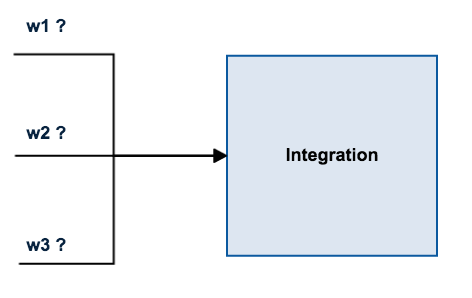
\includegraphics[scale = 0.4]{INT.png}
	\end{center}
\end{frame}
\begin{frame}
	\begin{block}{Planning}
		\begin{itemize}
			\item UvA is wholly responsible in planning body pose policies.
			\item Does planning have different priorities in social occasions?
			\item Do we plan myopically? 
			\item Collaborating with UPO on Navigation.
			\item How will the two be regulated?
		\end{itemize}
	\end{block}
	\begin{center}
		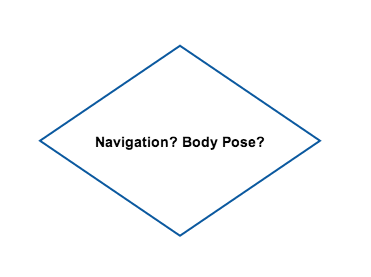
\includegraphics[scale = 0.35]{PLAN.png}
	\end{center}
\end{frame}

%% CURRENT RESEARCH INTERESTS -----------------------------------------------------------------------------------------------------------------------------------------------
\section{Current Research Intrests}
% IRL
\begin{frame}{Inverse Reinforcement Learning}{Definition}
	\begin{block}{Given:} 
		\begin{enumerate}  
			\item Measurements of an agent's behaviour over time, in a variety of circumstances
			\item Sensory inputs to the agent.
			\item A model of the Environment.
		\end{enumerate}
	\end{block}
	\begin{block}{Determine:} The reward function $R(s,a)$ being optimised. 
	\end{block}	
\end{frame}
\begin{frame}{Inverse Reinforcement Learning}
	\begin{itemize}
		\item An \textbf{apprentice} observes a state action trajectory $[(s_1,a_1), (s_2,a_2), ... ,  (s_T,a_T)]$  from an \textbf{expert}.
		\item $MDP_E = <S,A,T,\gamma,R>$ - R is hidden from the apprentice.
		\item Usually $R =w^T\phi(s,a)$ 
		\item So the IRL algorithm takes as input the trajectory and outputs the feature weights \pmb{w}.
		\item These are used by the apprentice to mimic and generalise the expert's preferences.
	\end{itemize}
\end{frame}
\begin{frame} {Inverse Reinforcement Learning}
Algorithms work by choosing weights to match certain trajectory statistics e.g:\\
\textbf{Feature Expectation} : $\Phi_E = \frac{1}{m}\sum_{m=0}^M\sum_{t=0}^T \phi(s_t,a_t)$\\
\textbf{Likelihood} : $P(s_{1-T},a_{1-T}|\pmb{w})$
	\begin{block}{Problems}
		\begin{itemize}
			\item Many Reward functions will cause the observed behaviour. Additional constraints are many times used.
			\item Each iteration usually requires solving the MDP.
		\end{itemize}
	\end{block}
\end{frame}
% SURVEY
\begin{frame}{Many Approaches}
	\begin{block} {Max margin + Projection}
		Ng and Abbeel (2004) successfully applied their algorithms on simulated car driving.
	\end{block}
	\begin{block} {Max Entropy IRL}
		Ziebart et al (2010) added extra disambiguating constraints and applied to route prediction.
	\end{block}
	\begin{block}{Maximum Margin Planning}
		Ratliff et al (2006) Posed the problem as a Structured Classification. Again applied to route prediction
	\end{block}
	Many more....But.
\end{frame}
% PARTIAL OBSERVABILITY TODO add tiger problem slide. add not clear aim of IRL feature expectation
\begin{frame}{Partial Observability in IRL}
	\begin{block}{Observation 1:} All literature assumes the expert and apprentice have the same observational capabilities. \end{block} % explain this better
	\begin{block}{Observation 2:} No principled reason why IRL is better than imitation. \end{block}
	\begin{block}{Motivation} Partial observability is possible the case in TERESA. e.g: 
		\begin{itemize}
			\item The Pilot-Expert only senses through a camera.
			\item The Robot has 360 degree laser range finding capabilities.
		\end{itemize}
	\end{block}
	\setbeamercolor{postit}{fg=white,bg=MyBlue}	
	\begin{beamercolorbox}[sep=0.5em,wd=10cm]{postit}
		=> What are the implications of observability mismatch in IRL?
	\end{beamercolorbox}
\end{frame}

\begin{frame}{Extreme No 1}{Tiger Problem}
	\begin{center}
		Apprentice $\rightarrow$ partial observability \textbf{|} Expert $\rightarrow$ full observability\\
		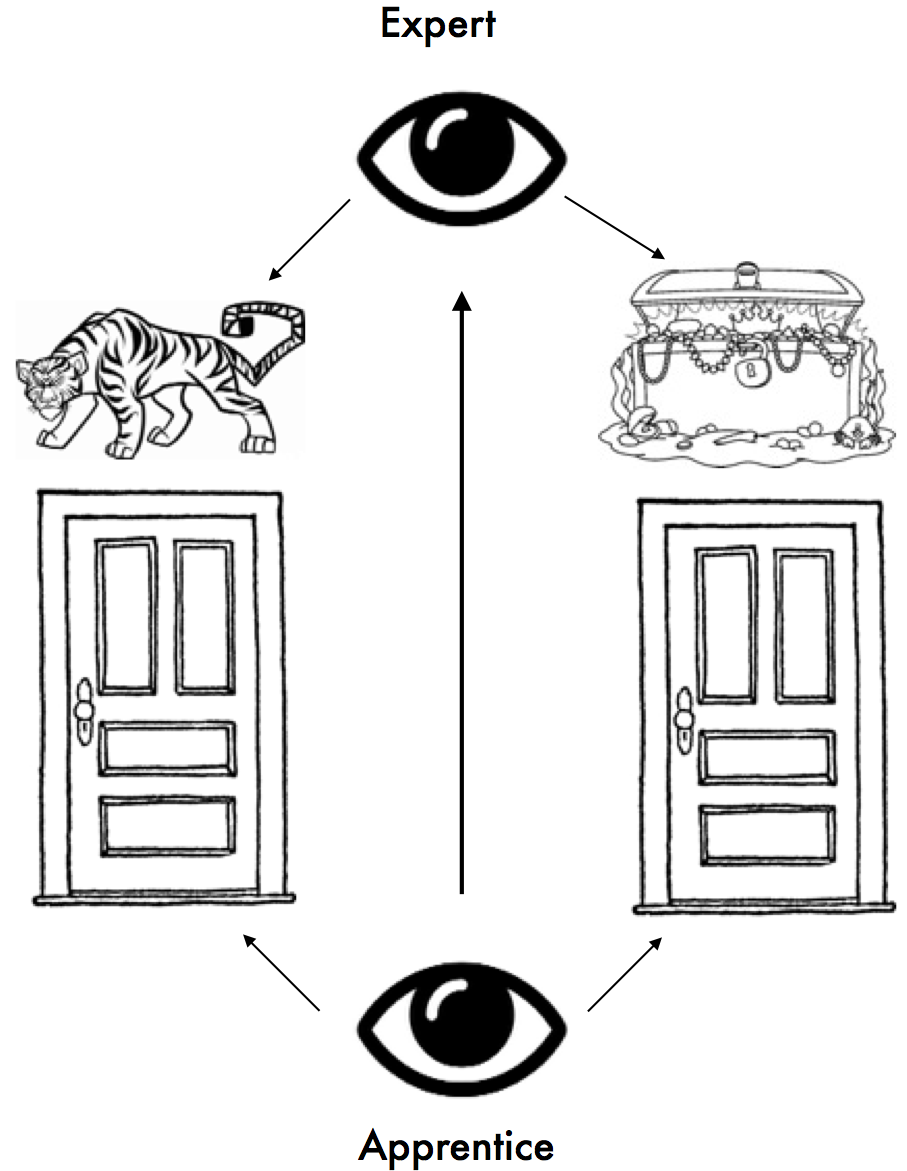
\includegraphics[scale = 0.35]{Tiger1.png}
	\end{center}
\end{frame}


\begin{frame}{Extreme No 1}
	Apprentice $\rightarrow$ partial observability \textbf{|} Expert $\rightarrow$ full observability\\
	\vspace{-1mm}
	\begin{center}
		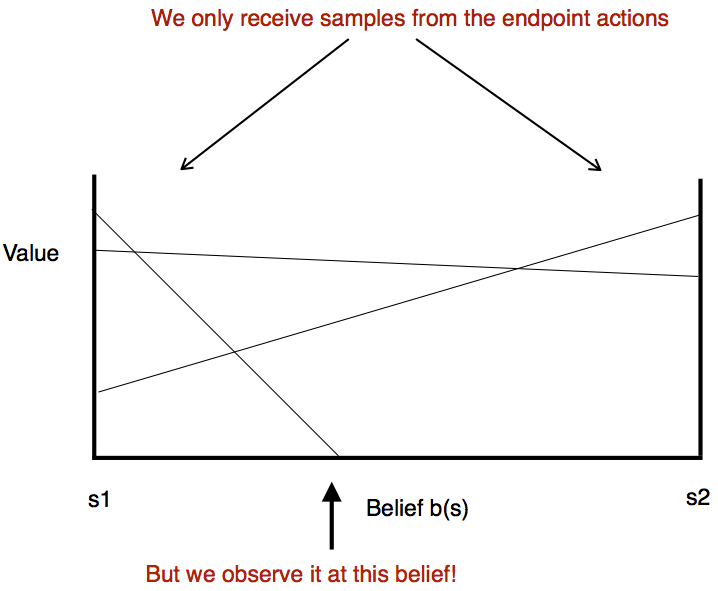
\includegraphics[scale = 0.45]{Diagram.png}
	\end{center}
	\vspace{-4mm}
		\begin{itemize}
			\item We now receive belief-action trajectories $[(b(s)_1,a_1),(b(s)_2,a_2),...,(b(s)_T,a_T)]$
			\item False information about what to do in uncertain belief states.
			\item Less information about what the expert is trying to do!
		\end{itemize}
	\setbeamercolor{postit}{fg=white,bg=MyBlue}	
\end{frame}

\begin{frame}{Extreme No 1}{Possible Solutions}
	\begin{enumerate}
		\item Perform forward-backward procedure on beliefs. This will push our samples to the extremes of the simplex.
		\item Assume a dual controller for the Apprentice.
			\begin{itemize}
				\item The information gathering part of the Reward function is given.
				\item The control part of the Reward function is learned from the expert trajectories.
			\end{itemize}
	\end{enumerate}
\end{frame}


\begin{frame}{Extreme No 2}{Tiger Problem}
	Apprentice $\rightarrow$ full observability \textbf{|} Expert $\rightarrow$ partial observability\\
	\begin{center}
		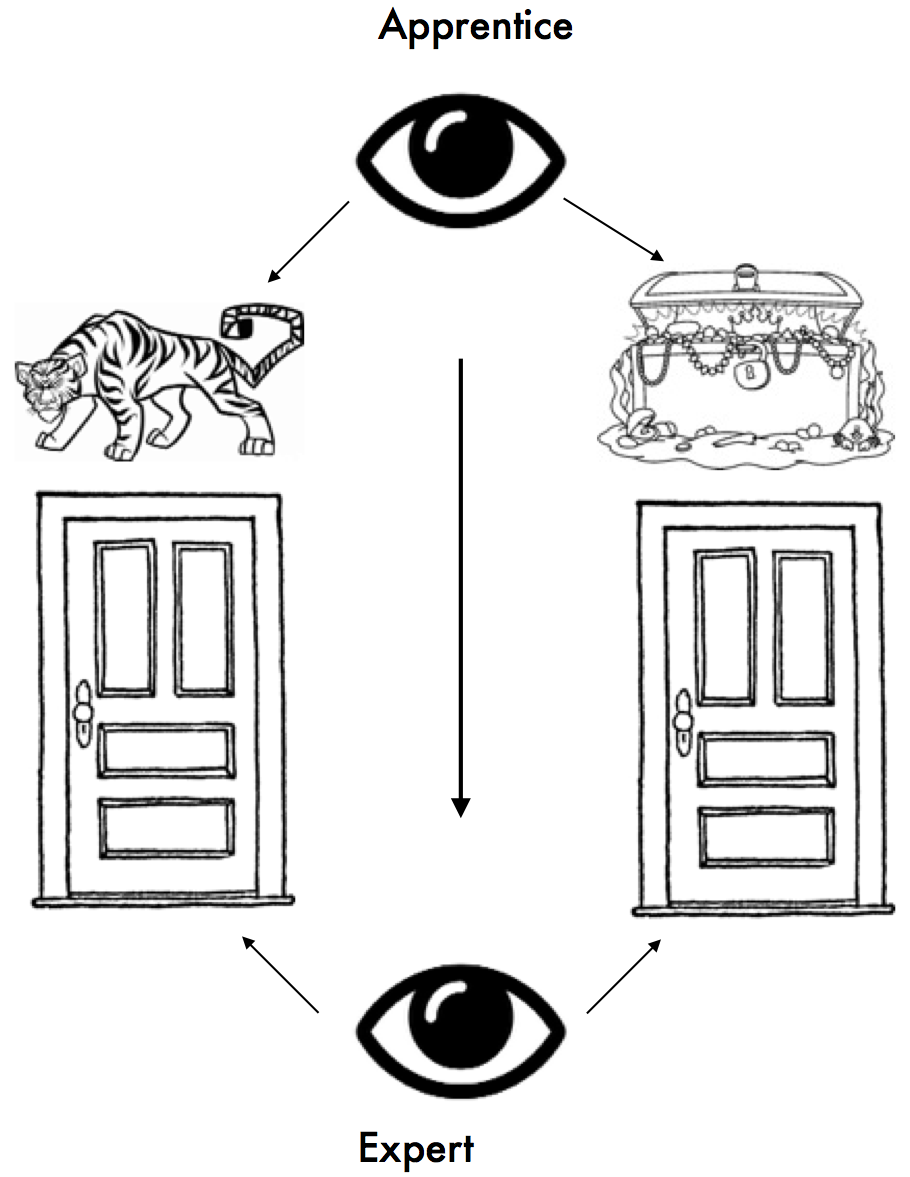
\includegraphics[scale = 0.35]{Tiger2.png}
	\end{center}
\end{frame}

\begin{frame}{Extreme No 2}
	Apprentice $\rightarrow$ full observability \textbf{|} Expert $\rightarrow$ partial observability\\
	\vspace{-1mm}
	\begin{center}
		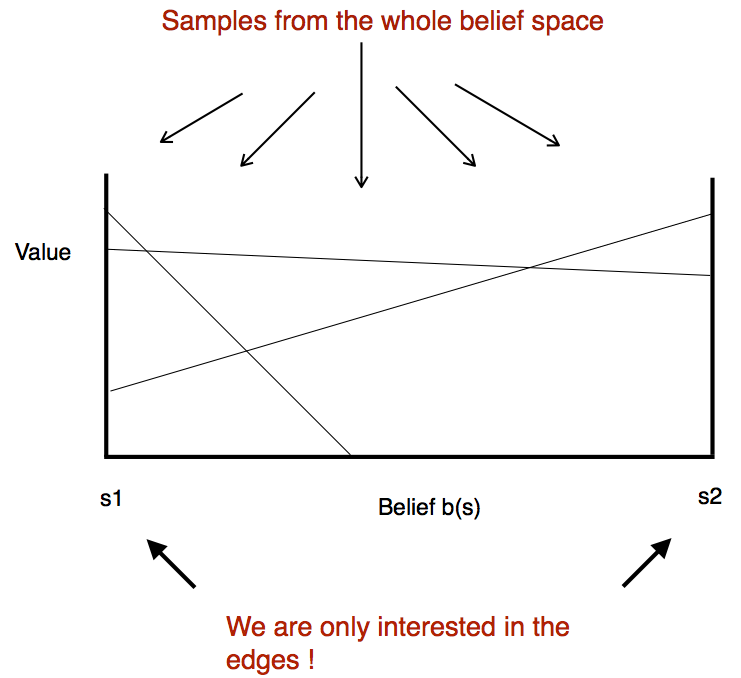
\includegraphics[scale = 0.42]{Diagram2.png}
	\end{center}
	\vspace{-5mm}
		\begin{itemize}
			\item We now receive state-belief(belief)-action trajectories $[s_1,b_A(b_E(s))_1,a_1),(s_1,b_A(b_E(s))_2,a_2),...,(s,b_A(b_E(s))_T,a_T)]$
			\item We don't want to know what to do in uncertain belief states.
			\item Less information about what the expert is trying to do!
		\end{itemize}
	\setbeamercolor{postit}{fg=white,bg=MyBlue}	
\end{frame}

\begin{frame}{Extreme No 1}{Possible Solutions}
	\begin{enumerate}
		\item Perform forward-backward procedure on beliefs of beliefs. Again, this will push our samples to the extremes of the simplex.
		\item Assume the expert is using a dual-controller.
			\begin{itemize}
				\item The information gathering part of the Reward function is given.
				\item The control part of the Reward function is learned from the expert trajectories.
			\end{itemize}
	\end{enumerate}
\end{frame}

\begin{frame}{Partial Observability IRL}{Conclusions}
	\begin{centering}
	\setbeamercolor{postit}{fg=white,bg=MyBlue}	
	\begin{beamercolorbox}[sep=0.5em,wd=10.5cm]{postit}
		We are no longer trying to replicate the expert's behaviour!
	\end{beamercolorbox}
	$\Rightarrow$ This provides a much more clear motivation for IRL!
	\vspace{9mm}
		\setbeamercolor{postit}{fg=white,bg=MyBlue}	
	\begin{beamercolorbox}[sep=0.5em,wd=7.5cm]{postit}
		As posed, the problem seems unsolvable.
	\end{beamercolorbox}\\
	$\Rightarrow$ We need to make extra assumptions and approximations!
	\end{centering}
\end{frame}

\/*


% PROJECT PARTNERS AND WORKPACKAGES 
\begin{frame}{Partners and Work-Packages}
	\begin{columns}
		\begin{column}[t]{2cm}
		
\includegraphics[scale = 0.1]{UVA.png}
		\end{column}
		\begin{column}[t]{2cm}
		
\includegraphics[scale = 0.2]{GIRAFF.jpg}
		\end{column}
		\begin{column}[t]{2cm}
		
\includegraphics[scale = 0.8]{UPO.png}
		\end{column}
		\begin{column}[t]{2cm}
		
\includegraphics[scale = 0.3]{IMP.jpg}
		\end{column}
		\begin{column}[t]{2cm}
		
\includegraphics[scale = 0.3]{TWENTE.jpg}
		\end{column}
	\end{columns}
			\begin{itemize}
				\item \textbf{WP1} : Project Coordination and Management - UvA.
				\item \textbf{WP2} : Detecting and Undestanding Social Behaviour - Imperial, University of Twente.
				\item \textbf{WP3} : Socially normative Human-Robot Interaction - University of Twente.
				\item \textbf{WP4} : Social Navigation - Universidad Pablo de Olavide (UPO)
				\item \textbf{WP5} : Learning Social Skills - UvA.
				\item \textbf{WP6} : Integration, deployment, evaluation - Giraff.
			\end{itemize}
\end{frame}
\begin{frame}{Example}

\end{frame}

\subsection[Kurzversion des ersten Unterabschnittstitels]
{Erster Unterabschnittstitel}

\begin{frame}{�berschriften m�ssen informativ sein.\\
    Korrekte Gro�-/Kleinschreibung beachten.}{Untertitel sind optional.}
  % - Eine �berschrift fasst einen Rahmen verst�ndlich zusammen. Man
  %   muss sie verstehen k�nnen, selbst wenn man nicht den Rest des
  %   Rahmens versteht.

  \begin{itemize}
  \item
    Viel \texttt{itemize} benutzen.
  \item
    Sehr kurze S�tze oder Satzglieder verwenden.
  \end{itemize}
\end{frame}

\begin{frame}{�berschriften m�ssen informativ sein.}

  Man kann Overlays erzeugen\dots
  \begin{itemize}
  \item mit dem \texttt{pause}-Befehl:
    \begin{itemize}
    \item
      Erster Punkt.
      \pause
    \item    
      Zweiter Punkt.
    \end{itemize}
  \item
    mittels Overlay-Spezifikationen:
    \begin{itemize}
    \item<3->
      Erster Punkt.
    \item<4->
      Zweiter Punkt.
    \end{itemize}
  \item
    mit dem allgemeinen \texttt{uncover}-Befehl:
    \begin{itemize}
      \uncover<5->{\item
        Erster Punkt.}
      \uncover<6->{\item
        Zweiter Punkt.}
    \end{itemize}
  \end{itemize}
\end{frame}


\subsection{Zweiter Unterabschnittstitel}

\begin{frame}{�berschriften m�ssen informativ sein.}
\end{frame}

\begin{frame}{�berschriften m�ssen informativ sein.}
\end{frame}

\section*{Zusammenfassung}

\begin{frame}{Zusammenfassung}

  % Die Zusammenfassung sollte sehr kurz sein.
  \begin{itemize}
  \item
    Die \alert{erste Hauptbotschaft} des Vortrags in ein bis zwei Zeilen.
  \item
    Die \alert{zweite Hauptbotschaft} des Vortrags in ein bis zwei Zeilen.
  \item
    Eventuell noch eine \alert{dritte Botschaft}, aber nicht noch mehr.
  \end{itemize}
  
  % Der folgende Ausblick ist optional.
  \vskip0pt plus.5fill
  \begin{itemize}
  \item
    Ausblick
    \begin{itemize}
    \item
      Etwas, was wir noch nicht l�sen konnten.
    \item
      Nochwas, das wir noch nicht l�sen konnten.
    \end{itemize}
  \end{itemize}
\end{frame}
*/

\end{document}


